\chapter*{Editorial}

Looking back over the caving exploration between 2007 and 2012 it almost
seems like it was a pre-ordained story. Living it, it never seemed like
this, rather a more confused and complicated picture, individuals actors
without a script, pulling together in some vague direction but towards
perhaps an achievable objective.

If exploration were a rational expenditure of efforts towards a known
end, the scenes would be rather more simple to describe - we realised
how close we were to the connection of Vrtnarija and Kavkna Jama (M2)
after more carefully analysing the 2007 ``Kill 'em All'' survey data. To
pursue this, we rebolted and rerigged Kavkna Jama in 2008, while
exploring on the other side in Vrtnarija. In 2009 we established a camp
in Vrtnarija at the nearest suitable point to the closest approach, and
used it to massively increase our time at the pushing front. In 2010,
2011 and 2012 we camped deeper in Vrtnarija, while pushing Kavkna Jama
from the surface both during the Summer and on Autumn / Winter trips. In
2012 we connected the systems, forming the longest cave system in
Slovenia, and one in which the vast majority of cave passage is at
depths greater than 500 m.

However, this isn't the real story of exploration. Rather, it is the
story of the people involved that is the true history of Migovec. For
the connection was not made in the obvious location between Kavkna Jama
and Vrtnarija, but down at 650 m of depth, as the result of yet another
successful, to the point of routine, pushing trip. Motivated by the
connection target, during 2008 we flung ourselves into the exploration
of Captain Kangaroo, Vrtnarija. At the grim pushing front were the
youngsters, highly motivated but lacking the experience to go deep.
Lacking in time at the pushing front we determined to go back and camp
in 2009.

``The art of roughing it is in smoothing off the edges.'' Stories of
draughty campsites, cassette players slurring to an undignified
quietness, shivering through the night, and unlabelled plastic bags of
miscellaneous white powder were retold by the experienced members, and
duly obsoleted by careful consideration of the logistics. We went back
with free standing tents, layers of fleece, MP3 players, modern
winter-mix gas stoves and LED fairy lights. We went back to stay, and
almost effortlessly pushed this tough branch of the cave down to 550 m.

This new generation of cavers, who cut their teeth in Captain Kangaroo,
suddenly found themselves with the endurance and know-how to
successfully explore at depth. Though the connection of the systems were
certainly still a major aim of 2010, 2011 and 2012 expeditions, we were
mainly there to push deep new cave passage. We re-established Camp X-Ray
(550 m deep) as our main base, and improved on it year after year till
it became a truly palatial location. And now that the going was once
again deep, we were rejoined by the more experienced members of our
club, for whom the prospect of another grim rift in Captain Kangaroo was
not suitably motivating. And as our collective abilities improved,
normality shifted. Exploring over multi-day camping trips, hot bunking
and the considerable feat of endurance just to reach and return from
these depths became standard practice. That which was just-possible the
year before became the standard trip, that which was beyond our reach
became achievable.

I am proud of the time that I have dedicated towards these expeditions,
and every moment spent with the people involved. There are others in the
club who have contributed very much more. We were all volunteers - we
did all this because we wanted to, but little would get done if we only
did things that were fun. Spending your free-time down caving stores
fettling kit is neither particularly enjoyable nor directly rewarding.
Carries in the hail and rain are arduous and unpleasant. I don't think
it is possible for this document to understate the sacrifice of time and
effort made by expedition members and friends. Forever lacking in
adequate funding and gear, unrecognised and often misunderstood, we have
achieved our exploration on a wing and a prayer.

This exploration report is dedicated to our many friends who assisted,
sponsored, carried, hosted and advised. You all contributed to the
achievements documented herein.

And so, Ninety-Nine years after Apsley Cherry-Garrard returned to South
Kensington with the Penguins Eggs, we return to our college with a minor
news story and a few pretty photos for their website. For those involved
in the exploration of Tolminski Migovec far more precious are the
memories of friendships formed deep within the Hollow Mountain.

We were always in the longest cave in Slovenia, we just hadn't realised.

\attrib{Jarvist Moore Frost}

\begin{verse}
We shall not cease from exploration  \\
And the end of all our exploring  \\
Will be to arrive where we started  \\
And know the place for the first time.  \\
Through the unknown, unremembered gate  \\
When the last of earth left to discover  \\
Is that which was the beginning;  \\
At the source of the longest river  \\
The voice of the hidden waterfall \\
\end{verse}

\attrib{T. S. Eliot}

\chapter{Vodna Sled: Slovenia 2010}

Vodna Sled 2010 was a clear success - in all we discovered 2.2km of new
passage, all below -500m, all in Vrtnarija using \textsc{Camp
X-Ray} (\textsc{Reloaded}, now a plush four bed camp at -550 m) as a
base. The majority of the discoveries lead from a horizontal series near
\textsc{Zimmer} chamber with numerous un-pushed leads for next year and
over 1.5 km of passage. Significant amounts of exploration also took
place in \textsc{Tolminska Korita} concluding with a connection to the
`deep' level at -653 m, and pushing the \textsc{Republica} streamway
from -744 to -802 m.

\section{Expedition Overview}

Twenty-two expedition members travelled from the UK for a total of 65
person-weeks in the field, with 88 person-trips in our callout roster.
Seventeen from the UK stayed at underground camp, along with six
Slovenes from the local JSPDT club, a total of 95 people-nights at camp.
All successful exploration took place on camping trips. This was the
first expedition for three first-year UK students, all of whom stayed at
underground camp and discovered significant quantities of new cave.

In all, the cave consumed a kilometre of rope for the rerigging of the
main pitch series, and newly explored sections left rigged (or with rope
pulled up) for 2011.

No work during the 2010 expedition went into M2 (Kavkna Jama), directed
towards forging a connection with Vrtnarija. However, during the early
Autumn two JSPDT trips capped through the tight rift at the very end of
the cave (\textasciitilde{}-390m), discovering and then descending a
\textasciitilde{}60m pitch.

The prospects for 2011 are extremely good. The extensive horizontal
development has led to the discovery and initial exploration of a number
of independent streamways and associated pitch series, in a horizontal
slice of the mountain we have never visited.

\begin{figure*}
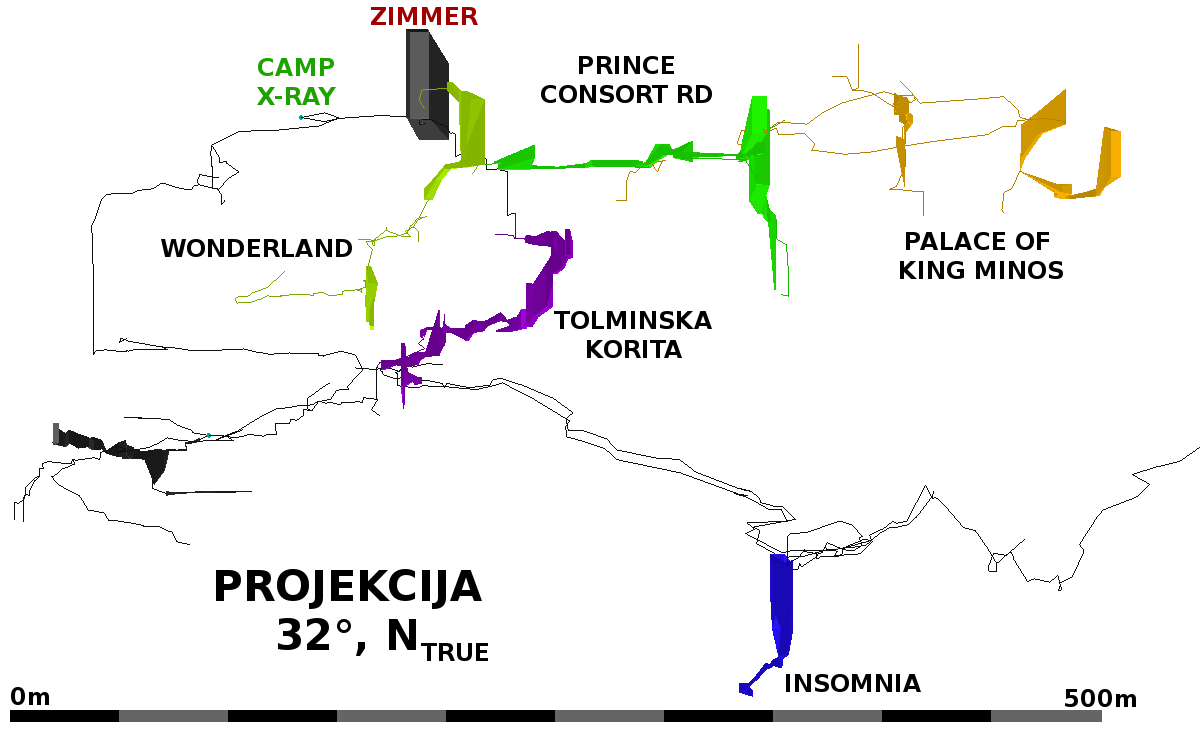
\includegraphics[width=0.85\columnwidth]{2010/2010_deep_vrtnarija_colour_coded_inverted_labelled}
\caption{Colour coded diagram of new cave discovered \& surveyed in 2010 in
Vrtnarija.}
\end{figure*}

\section{Expedition Findings}

The initial effort of the expedition was directed into setting up
underground camp. As the first pushing trips from this underground camp
came back with positive news, exploration based from camp (i.e.~deep in
Vrtnarija) quickly became the main focus of expedition effort. This came
at the cost of further work in bounce trips down Captain Kangaroo
(Vrtnarija, the likely connection region to M2) and M2 / SysMig itself.

The usual surface bashing continued, looking for new cave systems on the
plateau. A revisit was made to the area north of Kuk. This region is
heavily cratered with clear cave development, but the fear is that the
limestone is too broken and chossy for a human sized entrance.

We first visited this region with a serious aim of cave exploration in
2008, and returned in December 2009 on a `winter recce' by a two person
team with ice axe and crampons to identify which surface features were
actively linked into extensive underground systems through the holes
blown in the snow. Several more entrances were identified during this
recce, ones that were likely to be continued to be ignored in the summer
due to their unusual position.

These entrances were relocated this summer, but no new descents were
made.

\subsection{Leopard --- 1.5 km of new passage}

\begin{figure*}
\centering
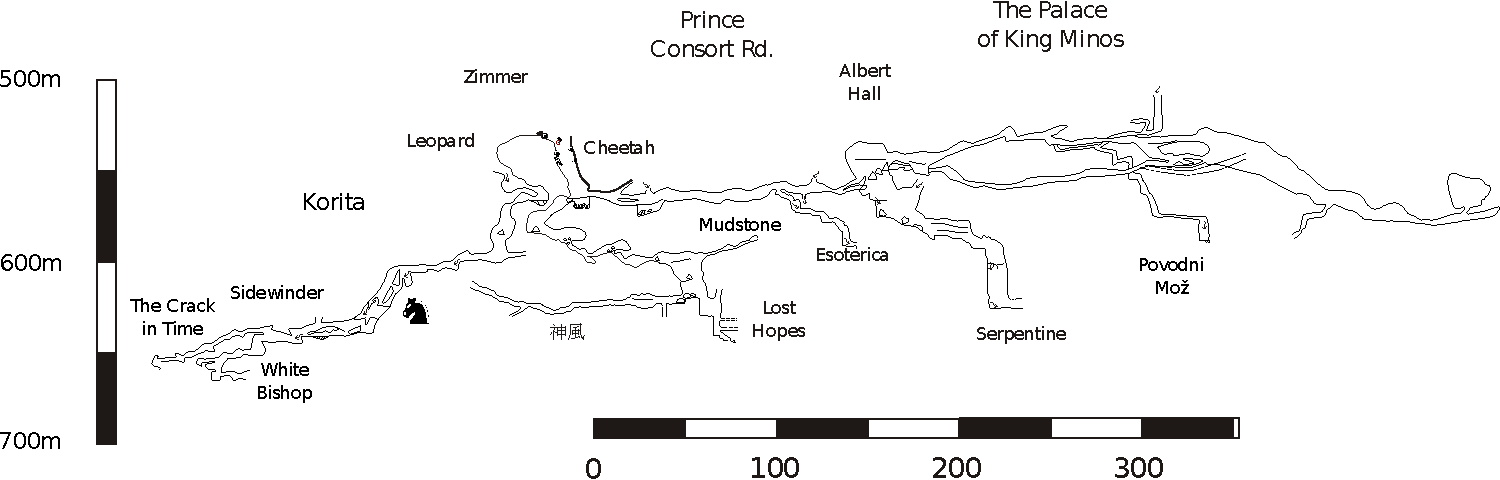
\includegraphics[width=0.9\columnwidth]{2010/2010_new_stuff_extended_extraction}
\caption{Extended elevation of new cave discovered in \textsc{TOLMINSKA KORITA} and \textsc{PRINCE
CONSORT} during 2010 Expedition.}
\end{figure*}

Leopard became the great focus of exploration this year. This lead (a
window off Zimmer chamber, now a 15m `up' pitch) had also been
originally discovered in 2001, but the drop that it led to had lain
untouched since then. This was partially due to its loose and muddy
nature, but also that deep exploration had concentrated on good leads
elsewhere (most particularly the lower Vrtnarija level accessed with the
bottoming of \textsc{Big Rock}). This took several sessions of rigging
and gardening to successfully conquer, and is is now named Cheetah
(P35m), because of the sense of having cheated death that it engenders
on passing. There are several windows off Cheetah, which are definitely
promising, although not easily accessible because of the broken nature
of the rock.

At the bottom, it intersects a horizontal, fossil passage, which has
been explored in three main horizontal parts:

Wonderland (heading South) linking into Rolling Stones, Surprise,
Mudstone Traverse, Kamikaze and finally Lost Hopes. Mainly dry with
large breakdown chambers.

Prince Consort Road (heading North) was initially pushed to
\textsc{The Albert
Hall} (from where the \textsc{Serpentine} meander leads off to the
\textsc{It
Will Rain for a Million Years} pitch), bisects three streamways (one of
which was pushed and forms the Esoterica series) and includes
considerable calcite formations.

From \textsc{The Albert Hall} a climb was made into the
\textsc{Palace of King Minos}. This passage is complex, and side
branches have neither been fully explored nor surveyed. The known
passage leads via Minotaur Rift to terminate in the Queens Bed Chamber
where the draught disappears towards the ceiling.

Together this passage leading off from Cheetah has been explored to over
1.5 km in length, and we are sure that more is yet to be found.

A significant volume of air flows through these regions, indicating that
there may be further developments.

\subsection{Wonderland}

Wonderland is the southern-most of the horizontal development, leading
directly off from Cheetah. It was pushed to a small pitch dropping into
a boulder filled chamber, Rolling Stones, which was the limit of the
first exploration trip due to the lack of rope. This chamber is situated
right below Zimmer, about 40m deeper. There is a further, as yet
unpushed, pitch going down between the large, seemingly unstable,
boulders on the floor.

A happen stance crawl behind some boulders led to further drafting
passage (Hidden Surprise), which, after traversing another chamber and
crawl, finishes in a chamber with a massive hole in the floor (Kamikaze
pitch). The passage continues on the far side of the pitch (traversed on
mud along the left wall), however, due to the collapsed ceiling, these
developments are almost two-dimensional (Mudstone Squeeze). The squeeze,
which is filled with interesting fossilised mud formations, was pushed
to the limits of comfort, although it still continues.

Kamikaze consists of a series of small ledges. From the second ledge a
tell tale breeze led to an interesting bedding plane crawl pushed upwind
but still untouched downwind. The pitch was bottomed (Lost Hopes),
wherein an inlet was followed down a 10m pitch to a series of squeezes
and rifts which quickly became tight. There is a ledge halfway down Lost
Hopes, with a perhaps larger abandoned rift.

These three leads (Kamikaze, Mudstone, Lost Hopes) are of interest as
they now form the most Easterly extent of Vrtnarija at depth, seeming to
`spear' through the large N-S geological feature that contains the
majority of the horizontal passage.

The whole area of Wonderland is extremely dry, quiet and rather spacious
in its scope. It is particularly reminiscent of the higher level passage
in the Easegill system, Yorkshire.

\subsection{Prince Consort Road}

Prince Consort Road is the passage going north from Cheetah. Several
streams intersect it and some formations have been found there. The
discovery of stalactites covered with helictites proved particularly
exciting! The passage leads to a small boulder choke which was easily
surpassed and led to a large chamber (the Albert Hall). Before the
Albert Hall, three apparently unique streamways have been found:

One intersecting the passage along a traverse (water chokes into boulder
floor), then around a small chamber at about halfway to Albert Hall, on
a corner of the main massage approximately 2/3 of the way to the Albert
Hall a small rift to the east, and a nice white-sanded water inlet to
the west. The latter leads to an unpushed pitch under the main passage,
there is a cairn and note mentioning the lead. Of these, only the second
has been pushed, into the Esoterica series. Strangely this wet, tight
rift has only been visited once during the expedition, even though it is
still going!

In the Albert Hall two streams enter the chamber from on high (the
ceiling was measured as being over 30m up, by laser disto) and join into
a rather beautiful spacious vadose streamway (The Serpentine).
Serpentine was pushed and leads to another split pitch (It Will Rain for
a Million Years \textemdash{} pushed during a continuing flood pulse).
At the bottom of It Will Rain pitch the stream continues and has not
been explored.

\subsection{The Palace of King Minos}

North from the Albert Hall a muddy climb lead to The Palace of King
Minos. This passage and its continuation (The Minotaur Rift) has some of
the most beautiful formations found on Migovec to date, in particular
fine walls of calcite, gypsum and aragonite crystals, mud formations and
weird soot encrusted floors. The Palace has a labyrinthine nature with
several passages leading back to Albert Hall, the largest loop of which
was named Ouroboros

The passage has a classic large phreatic lozenge shape, with some parts
undercut by fossil vadose passage. Near the start of the passage a
significant breeze blew through a small hole. This was enlarged and
found to lead to a small phreatic tube which bizarrely led into an
active vadose streamway (Povodni Mo\v{z} \textemdash{} Water Nymph).
Povodni Mo\v{z} has been pushed upstream to a large active aven (and
smaller dry parallel shaft), and downstream to a sump (approximately
2mx2m in size in the corner of a small chamber and taking the small
flow) and has hence been derigged.

Continuing along the main Palace passage several horizontal tubes have
been explored which lead back into the main passage, though not all have
been entered in the survey. Eventually the main route leads to a high
and wide rift (Minotaur Rift \textemdash{} 20m high, 60m long) beyond
which the best formations are to be found. This passage has a few
interesting leads in it: a high, dry, circular, muddy window to the
right of the passage near a tiny inlet, 2 small tubes leading off the
main passage which both need a little mechanical persuasion.

The chambers beyond Minotaur Rift are spacious and display massive
amounts of crystal formation on all available surfaces --- there is
white `popcorning' almost everywhere, with regions of more intricate
needle and feather formations. The chambers decay into a crawl, which
almost unbelievably is over a smooth calcite floor. This leads to a
classic boulder choke gallery (choking at the end). On the left a small
boulder choke climb leads to the Queens Bed Chamber. In this large room,
the draught appears to disappear up towards the ceiling - both ends of
the chamber are potential climbing projects (\textasciitilde{}+20m).

The region is extremely reminiscent of Ogof Ffynnon Ddu II in Wales.

\section{Tolminska Korita}

This lead of Zimmer chamber had been discovered in 2001 but had lain
unexplored until last year, when the first few pits of the active
meander were pushed to a larger pitch. Korita developed into cascades of
active pitches (Black Knight series) to a duck. The duck was soon
bypassed by a 5m free climb into old phreatic level.

The passage beyond soon diverges into two continuations:

\subsection{Sidewinder, Crack in Time}

The higher dust filled dry phreatic level (Sidewinder, Crack in Time)
connects into \textsc{Envy} in the low level via free climbs and two
small pitches. It is not particularly surprisingly that the `Crack in
Time' was not explored from below, as the connection is made by a long
body-sized crawl above a thin (5 cm) crack connecting to known passage
(Envy), which happily pops out at the top of a obscure 3 m free climb.
Connecting into a 2004 era permanent survey station, Korita now forms a
second loop in Vrtnarija, forming Vrtnarija into a figure-8 shape with
Friendship Gallery at the waist.

\subsection{White Bishop, Stalemate}

The active streamway descends two 10-15 m pitches connected with a
spacious meander incorporating free climbable cascades, before ending in
an impassable rift (-662 m).

This water disappears into `blank mountain' on our survey, but would
require considerable effort to progress, and Korita was thus derigged.

\section{Roaring Floor Tease (Muddy Window off Happy Monday)}

This was regained by bolt climbing from the bottom of Happy Monday to
regain the Muddy Window. The climb in the mud chamber was made, but
quickly led to a large boulder blocking the way. A tight rift taking a
large draught was left unpushed. Progress is believed to require
expansion.

Similarly the traverse to an inlet on Falls Road, and the continuation
of Falls Road itself was left unpushed. A small dig was made in
Friendship gallery beyond Prima junction, which led to a small unpushed
pitch above a stream.

\section{Deep Leads (Below \textsc{Big Rock Candy Mountain})}

\subsection{Insomnia - Republika Streamway}

Last year a `written off' streamway (Republika, leading from Red Cow)
was found and pushed upstream to an aven fed watershed, then down the
other limb to a rift pitch.

With the promise of being one of the deepest points of the cave a return
in 2010 was obligatory. The pitch was found to be 41m and was pushed
down a continuing active rift (Insomnia). The end is now only 4m higher
than Colorado Sump (the deepest known point of Vrtnarija). Since the
limit of exploration is above a small 4-5m pitch it is understood that
in 2011 this will inevitably become the deepest passage in the system,
and the signs are good for continuing development of depth. The end is
802m below the entrance of Vrtnarija, but the M2 (Kakna Jama) entrance
is 75 m higher still, and a connection between the systems would make
this point -877m deep overall, with potential for further depth
extension.

\subsection{Balamory}

A return to Balamory was thwarted by lack of rope of the exploratory
party (one more pitch than expected on route), but the team made good
use of the trip to the depths by recovering the camping mats from the
deep 2004 camp (The Fridge, near Cactus Junction), and prospecting for
other leads with some success.

\section{Original Exploration Stories}

\subsection{Pushing Insomnia}

I had travelled down to T'min to clean and get over the cabin fever that
develops over the weeks of life on the Plateau. That night, after a slap
up meal and a few bruskies, Jan arrived and we had a great evening of
beer and bullshit. After the beer, we passed on to the whiskey and the
bullshit got increasingly epic. ``The leads at the bottom of Red Cow are
going to make GW deeper'' I told Jan ``the next pushing trip will
definitely do it''. So after walking up the hill having dinner and a
little too much to drink at the bivi we set off for the night train.

Soon enough we are at camp and decide to keep going down, looking to
continue pushing the Republika lead. I must admit it took a lot of
strength not to push the leads that were already multiplying at the I
knew the way to Red Cow, having been there with Dan a few days earlier.
We soon got to the junction and followed the water upstream. Nice
caving, I start feeling the all familiar excitement: here come lots of
km of fresh cave!

At one small pitch I turn around and find Jan has disappeared. I turn
back to look for him and find him wandering in the wrong direction
towards the sump. Apparently he had fallen asleep and started wandering
off route. Shit maybe we are too tired for this? Meh! We get to the
pitch head for Republika, which I must admit is rather God forsaken and
wet and awful. We drop the pitch, I get the drill out and start rigging,
brain totally disengaged. As I am rigging I can feel the batteries
getting weaker and weaker. I guess there were a few too few bolts at the
bottom of the main drop and maybe some of the pitch heads could have
been a little neater. It certainly helps to cave with a tall bastard is
all I can say :D.

We reach the bottom of the main new pitch and it's a rather God forsaken
wet and damp place. The water keeps going down along some immature
passage. We follow the water, noting at least one unlikely but unchecked
possible side passage. A few hand lines are placed here and there and
the drill battery finally dies. Just as well as the last pitch we get to
looks like a right nightmare: really tight pitch head etc. By this point
we realise it's super late and we are almost certainly going to miss our
callout. Time has gone in a blur, we are probably not 100\% there
mentally to be honest. Still might as well survey out.

The way out is not very remarkable. We bump into Tetley at the top of
Big Rock. He is not too worried, but apparently Gergely was hoping we
were crumpled up in a heap somewhere so he could come and rescue us.

\attrib{James Kirkpatrick}

\subsection{More Horror with Jan.}

The next night we get up and decide to do some pushing. The whole day is
marred by the fact that - once again - we promised not to push the
obvious continuation from Albert Hall. So we decide to have a random
bimble around. We try looking for alternative ways around the Albert
Hall. No success. Somehow we end up pushing a lead from the right of the
passage leading to the Albert Hall (right looking towards the Albert
Hall!).

The passage is small and bends under the main route. It is wet and
rather grotty. We drop a pitch or two of utter horror and eventually
turn around. Surveying out is awful. The book gets wet, my fingers are
too cold to hold the
instruments\footnote{The survey data had to be 'corrected' to avoid the survey self-intersecting due to backwards legs.}.
It sucks majorly. At least the passage gets a cool name: Esoterica. O,
and no-one has pushed the pitch where we stopped!
\footnote{Esoterica was not revisited until 2012, where a broken bolting driving prevented any additional pitches being descended. It remains a lead.}

\attrib{James Kirkpatrick}

\subsection{Happy days with Jan.}

On our last day together we went looking around the amazing passage that
we politely left for Dan and Izi. We smashed our way through the
entrance of what would become Po Vodni Mos, we looked at the Queen's bed
chamber, we pushed down some random tubes at the sides of the main route
(has anyone ever surveyed these I wonder, one of them went!). All in all
a super chilled day. No surveying and no water. And then we got back to
camp, watched some videos and drank a lot of whiskey, Happy Days!

\attrib{James Kirkpatrick}

\subsection{Balamory}

When James and I went to have a look at the bottom of Balamory on the
first day of our one-noght camping trip, we didn't make it to the target
as an unexpected first pitch used up too much of the rope that we had
taken with us.

However, as well as airflow going towards Balamory, there is also
airflow in the main passage above, beyond the point where the hole down
to Balamory leads off so here are two leads in that area there that are
worth looking at.

The upper lead \emph{does} need some way of climbing across a pit to a
ledge covered in loose crap (maybe a bolt traverse round one of the
walls, though I can't remember how much good rock there was in that
area. Subsequent email exchanges on the subject do seem a bit vague as
to exactly what was done, and whether the upper passage had actually
been boldly examined or not (Clewin was bold somewhere round there, but
it wasn't certain where), but anyone going to potentially move/split the
boulder down Balamory (I think it was supposed to be down the third of
the three possible `second pitches') down should also probably plan to
look at the upper passage continuation, especially if they have a
drill/bolts to help with climbing/traversing belays.

On the way back from this little trip, after grabbing some stashed
karrimats from the old camp, that the black black hole across Big Rock
was noticed.

The next day, James and I went to the new stuff below Leopard/Cheetah,
but since we were doing a push-then-out trip, rather than going to the
far end of the `half' where most of the action was, we went in the other
direction from the pitch bottom to do some work relatively close to
camp, carrying on where Gergely+???? had left off at the Hidden Surprise
pitch.

Gergely had dropped the first section of the pitch to an obvious ledge
and followed the ledge to horizontal passage that soon died. James and I
were to descend the shaft from the ledge, but it immediately became
clear the drill wasn't working and so we had to resort to spits, with
James bolting while I waited on the ledge.

Fairly soon the bolt (bolts?) was in and James had descended to a large
boulder-covered ledge part-way down the large shaft, where I could
safely join him. Some of the boulders were rather large, with gaps
between them or between them and the wall large enough to climb down and
move around in. While James did the business with the next spit, I
wandered around between the boulders to keep busy. Where the boulders
met the wall, the wall was somewhat overhanging, and from the lowest
easily-accessible place near where I had first climbed down, it was
possible to look between the boulders marking the lower limit of easy
movement and the wall to see a few metres away/down to where the wall
seems to meet the proper floor of the ledge, where there was a layer of
white rock flour, with some potentially human-sized space between me and
it though with no obvious way to get there.

From where I was, looking along the wall `clockwise', it also looked
like there was a space of some sort ahead of me horizontally, but
getting to it didn't look very nice, and after all, I was just in a pile
of boulders on a big ledge half-way down a pitch, not in a classic
boulder choke as such, so there seemed little point doing anything
borderline just to get to a slightly different place in the boulder
pile.

However, just as I was preparing to go back up and see how James was
getting on, I breathed out a large sigh, only to see it get sucked
horizontally away from me between wall and boulders and into the space I
had been looking into, which immediately aroused my curiosity.

To get into the space I could see required going horizontally through a
not-quite-body-sized vertically-rectangular gap with a short (1m) drop
on the other side. After removing all my SRT kit, and doing some work
with a convenient rock hammering edges off the boulder forming one side
of the slot to make the gap wider, and progressively blunting sharp
edges on the wall side as they proved awkward when attempting to get
through, it was possible to slowly and delicately post myself through
feet first and eventually emerge free on the other side.

Turning around, a short crawl led to a wider area under the overhanging
wall, and a view ahead to where the wall/roof sloped nicely down towards
into the floor to leave a wide bedding plane with clearly no way on.
Turning around somewhat disappointed, the main wall, which I had been
looking away from when I had initially turned round, was seen to have a
crawling-height hole in it, which, on approaching, it was clear most of
the draught was going into.

That hole led to a small chamber with a further hole leading in turn
into the side of a walking-height passage with a good breeze running
along it. The draught I had followed initially was clearly just a
tributary being sucked into the main airflow.

I quickly returned to James to tell him of the find, and we decided to
do a little surveying and exploration. We chose the upwind branch which
didn't run a great distance before ending in an upwards bedding-plane
slope ultimately blocked by a large slab in the bedding blocking
sideways movement into what appeared to be a chamber with a waterfall
entering. Capping or plugs/feathers would seem to be needed to shift
this blockage. On returning to our entry point, we looked the other way,
wondered how far the downwind passage went, but left it for someone else
to explore.

We hadn't found a great deal of length, but on the other hand, we had
left a decent going lead, and due to the combination of a misbehaving
drill making waiting cold and dull work and the luck of my breath
showing there was something worth looking at, had ended up finding quite
interesting passage in what must be one of the most unlikely of
situations.

Thinking partly of the initial nervousness with which I had slowly
posted myself between the boulders and the wall, but mainly of the
immense luck we had had with the draught, Kamikaze seemed like the
obvious choice of name for the discovery.

\attrib{Dave Wilson}

\section{Underground Logbook}

\section{Found in `AggregateofMig2007-2010.doc' : Jarv Typed up?}

Camp X-Ray Logbook: After about 6 hours of caving, finally made it down.
Met Gergely \& James on he way down as they were leaving the cave. Last
bolt before camp is horrible = needs rebolting / rerigging. 15cm lower
would be awesome. Built a tent at teh camp. Required some stone
movement. Mike got water, me \& Jarv built tent, kate = smoking. NEED
WEED! Should have thought about it before. Listening to Massive Attack
and getting Raptured. Oh yeah! Kate setting up sleeping space, Jarv went
to get more water.

Camp is getting established, looking forward to Worms World Party. Mike
= Cooking. Weed is really a missing resource. So far so good. About 5
metres from camp is a hole with water in it = able to hear, quickly got
established as peeing corner, hope its not a lead\ldots{} Nick

23/7/10 Nice snooze - super warm. Nicola snored like a trooper - just a
few minutes into the classic Black Adder session. Broken sleep -
particularly as Nicola got up for X2 piss. Awoken @ 10:30AM by the
beasts crawling up towards our pits. Tetley \& Myles rustled up some
hot-choc then wandered off down the continuing passage.

23.7.10 - 2:10pm MD + Tetley Entered Gardener's World
\textasciitilde{}6:20am. Made our way through, re-rigged zimmer on the
way. Arrived at camp at 10:30am + awakened JV, Mike, Kate + Niko.

Wandered around friendship gallery for hour or two. Found nice lead,
will investigate later. Sleep now.

23-7 2:20pm

It's good to be back in a sleeping bag at Camp X-Ray - seven years since
the last camp here. It's very comfy. I like the tent - some things don't
change though, Blackadder on the sound system, smash + tuna etc.
Hopefully we'll get some good pushing in tomorrow! Tetley

23-7 6:20pm James and Dan arrive for a quick visit before heading off to
push the muddy window 8:20pm Andy + Gergely arrive - I ignore them! Tet

23-7 10:30pm Fucking body won't fall asleep! Must have only had couple
of hours at most since Dan arrived\ldots{} Gergei + Andy turned up at
8ish + now, they have checked our Leopard a little. Tetley's bodily
functions are out of control! May bring some corks down for his
digestive tract next time. Anyway, now for some food + tea + hopefully
can stay awake till bedtime at noon! Myles.

23-7 11pm Myles and I share breakfast / dinner with Gergely + Andy. Fine
food! (Ed: Believe this was Tetley)

24-7 12:20 Breakfast with Tet \& Miles. Dan \& I will visit the lead we
killed yesterday (Muddy Window) \& survey it, then to Red Cow. James K

24-7 1:30pm MD Back in Camp for 2nd night. Pushed Tolminka today, good
lead, surveyed \textasciitilde{}8am. Some nice pitches. Covered in mud.
Listening to strange foreign music.

24-7 2:05pm Great push down Korita today - 8 bolts, surveying etc. IT'S
GOING GOING GOING\ldots{} GO THERE! (But try and avoid rigging future
pitches in or near the water\ldots{}) Andy + Gergely have left to push
Leopard - James + Dan to survey Muddy Window and then go for a jolly
below Big Rock. I've had a great day - thanks Myles. Time for a decent
seep. Tet

23:20 24/7/2010 James + Dan return on a high! 9hrs good kip in bed - I
feel good! forgot to say I had a shit yesterday\ldots{}. Tet
